L'intégration correspond au processus inverse de la dérivation. 
Parler des péripéties du calcul différentiel entre Leibniz et Newton au 17e ? 




Dans tout ce chapitre, $f$ et $g$ désignent deux fonctions continues sur un intervalle $[a, b]$.

\section{Primitives et intégrales}

\begin{Def}\textbf{Primitive}

On dit qu'une fonction $F$ est une primitive de la fonction $f$ 
sur l'intervalle $[a ; b]$ si la dérivée de $F$ est égale à $f$.\vspace{1em}

C'est-à-dire qu'on a pour tout $x \in[a ; b]$ :

$$
F^{\prime}(x)=f(x)
$$    
\end{Def}



\begin{Rmq} beaucoup de primitives

    Si la fonction $F$ est une primitive de $f$, alors pour n'importe quel nombre réel $k$, la fonction $F+k$ est aussi une primitive de $f$, .
\end{Rmq}

\newcolumntype{M}[1]{>{\centering\arraybackslash}m{#1}}

% Alignement visuel uniforme (hauteur fictive pour toutes les cellules)
\newcommand{\alignvis}[1]{\vphantom{\dfrac{1}{x^n}}#1}

\renewcommand{\arraystretch}{2.3} % Espace vertical entre lignes

\begin{center}
\begin{tabular}{|M{3cm}|M{3cm}||M{4cm}|M{4cm}|}
  \hline
  \textbf{Fonction $f$} & \textbf{Primitive $F$} & \textbf{Fonction $f$} & \textbf{Primitive $F$} \\
  \hline
  $\alignvis{k \in \mathbb{R}}$ & $\alignvis{kx + C}$ 
  & & \\
  
  \hline
  $\alignvis{x^n,\ n \in \mathbb{N}}$ & $\alignvis{\dfrac{x^{n+1}}{n+1} + C}$ 
  & $\alignvis{u'(x)\, u^n(x),\ n \in \mathbb{N}^*}$ & $\alignvis{\dfrac{u^{n+1}(x)}{n+1} + C}$ \\
  \hline
    $\alignvis{\dfrac{1}{x}}$ & $\alignvis{\ln |x| + C}$ 
  &
    $\alignvis{\dfrac{u'(x)}{u(x)}}$ & $\alignvis{\ln |u(x)| + C}$ \\
  \hline
    $\alignvis{e^x}$ & $\alignvis{e^x + C}$ 
  & $\alignvis{u'(x) e^{u(x)}}$ & $\alignvis{e^{u(x)} + C}$ \\
  \hline
  $\alignvis{\dfrac{1}{x^n},\ n \in \mathbb{N}^* \setminus \{1\}}$ & $\alignvis{\dfrac{-1}{(n-1)x^{n-1}} + C}$ 
  &
  $\alignvis{\dfrac{u'(x)}{u^n(x)},\ n \in \mathbb{N}^* \setminus \{1\}}$ &
  $\alignvis{\dfrac{-1}{(n-1)u^{n-1}(x)} + C}$ \\
  \hline
    $\alignvis{\cos x}$ & $\alignvis{\sin x + C}$ 
  &
    $\alignvis{u'(x) \cos(u(x))}$ & $\alignvis{\sin(u(x)) + C}$ \\
  \hline
    $\alignvis{\sin x}$ & $\alignvis{-\cos x + C}$ 
  &
    $\alignvis{u'(x) \sin(u(x))}$ & $\alignvis{-\cos(u(x)) + C}$\\
  \hline
    $\alignvis{\dfrac{1}{\sqrt{x}}}$ & $\alignvis{2\sqrt{x} + C}$ 
  &  $\alignvis{\dfrac{u'(x)}{\sqrt{u(x)}}}$ & $\alignvis{2\sqrt{u(x)} + C}$  \\
  \hline
\end{tabular}
\end{center}

Petit QCM sur des primitives ? 



\begin{Def}\textbf{Intégrale}

On appelle intégrale de $f$ entre $a$ et $b$ et on note
$$
\int_a^b f(x) \dx
$$
l'aire algébrique en unité d'aire délimitée par la courbe de $f$ et l'axe des abscisses prise entre $a$ et $b$.
\end{Def}
\begin{figure}[h]
\centering
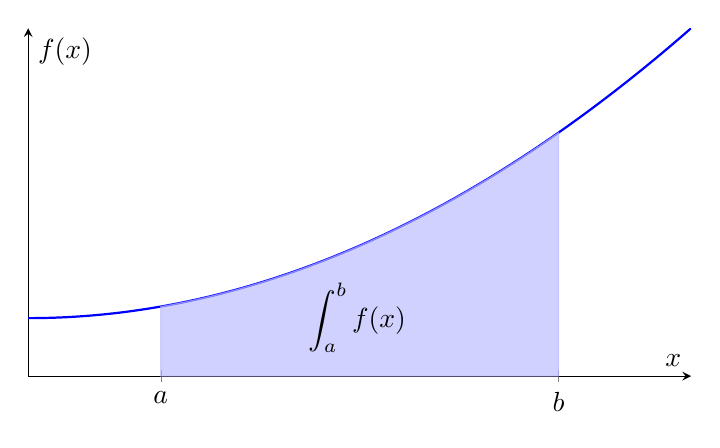
\begin{tikzpicture}
  \begin{axis}[
    axis lines = middle,
    xlabel = $x$,
    ylabel = {$f(x)$},
    xmin=0, xmax=5,
    ymin=0, ymax=6,
    xtick={1,4},
    xticklabels={$a$, $b$},
    ytick=\empty,
    domain=0:5,
    samples=100,
    clip=true,
    width=10cm,
    height=6cm,
  ]
  % Fonction
  \addplot[thick, blue, domain=0:5] {x^2/5 + 1};

  % Aire sous la courbe entre a=1 et b=4
  \addplot [
    domain=1:4,
    samples=100,
    blue!30,
    fill=blue!30,
    opacity=0.6
  ]
  {x^2/5 + 1} \closedcycle;

  % Annotation : intégrale
  \node at (axis cs:2.5,1) {$\displaystyle \int_a^b f(x)\,\dx$};

  \end{axis}
\end{tikzpicture}
\end{figure}

\begin{Thm}\textbf{Théorème fondamental de l'analyse}

Intégrale et primitive sont reliées par la relation fondamentale suivante : 
$$\int_a^b f(x) \dx=\big[F(x)\big]_a^b=F(b)-F(a)$$
où $F$ est une primitive de la fonction $f$.

La valeur de l'intégrale ne dépend pas du choix de la primitive.

\end{Thm}

\exo{Calculer les intégrales suivantes}

\begin{multicols}{3}
    \begin{enumerate}
\item[] $$\int_1^3 x \dx $$
\item[] $$\int_{-2}^1 6 x^2 \dx$$
\item[] $$\int_0^{\ln 3}\, e^{2 x} \dx$$
\item[] $$\int_1^3 \,\frac{2 x}{x^2+1} \dx$$
\item[] $$\int_{\pi / 4}^{\pi / 3} \, \frac{\cos x}{\sin x} \dx $$

\end{enumerate}
\end{multicols}

\hfill\break
\hrule
\hfill\break

On peut couper en deux le bloc suivant pour ne pas avoir cet espace vide .. 
\begin{Prop}Propriétés de l'intégrale
\begin{enumerate}
    \item L'intégrale sur un point est nulle $$\int_a^a f(x) \dx=0$$
    \item L'ordre des bornes est important $$\int_a^b f(x) \dx=-\int_b^a f(x) \dx$$
    \item L'intégrale d'une fonction positive est positive $$f \geq 0 \Rightarrow \int_a^b f(x) \dx \geq 0$$
    \item L'intégrale préserve l'ordre $$f \geq g \Rightarrow \int_a^b f(x) \dx \geq \int_a^b g(x) \dx$$
    \item Inégalité triangulaire $$\left|\int_a^b f(x) \dx\right| \leq \int_a^b|f(x)| \dx$$
    \item L'intégrale est linéaire pour la somme... $$\int_a^b f(x)+g(x) \dx= \int_a^b f(x) \dx+\int_a^b g(x) \dx$$
    \item ... et pour la multiplication par un scalaire $$
\forall \lambda \in \mathbb{R}\quad  \int_a^b \lambda f(x) \dx=\lambda \int_a^b f(x) \dx
$$
    \item Relation de Chasles
    $$\forall c \in[a, b]\quad \int_a^b f(x) \dx=\int_a^c f(x) \dx+\int_c^b f(x) \dx$$
\end{enumerate}
\end{Prop}

\section{Techniques d'intégration}
\subsection{Intégration par partie}

Le principe est d'exploiter la fameuse règle de Leibniz pour dériver un produit $$(u v)^{\prime}=u^{\prime} v+u v^{\prime}.$$ Il faut donc que les fonctions considérées soit dérivables et de dérivées continues pour être intégrables.

$$
\int_a^b f(x) g^{\prime}(x) \dx=\big[f(x) g(x)\big]_a^b-\int_a^b f^{\prime}(x) g(x) \dx
$$


Toute la difficulté réside dans le choix de $f$ et de $g^{\prime}$. Avec un peu de pratique il devient plus naturel.

\hfill\break

\exo{Calculer les intégrales suivantes}

\begin{multicols}{3}
    \begin{enumerate}
\item[] $\displaystyle \int_0^1 x e^x \dx$
\item[] $\displaystyle \int_0^{\pi / 2} x \cos x \dx$
\item[] $\displaystyle \int_1^e \ln x \dx$
\item[] $\displaystyle \int_0^1 x^2 e^{-x} \dx$
\item[] $\displaystyle \int_0^{\pi / 2} e^x \sin x \dx$
\item[] $\displaystyle \int_1^e x \ln x \dx$
\end{enumerate}
\end{multicols}

\hfill\break
\hrule
\hfill\break

\subsection{Décomposition en éléments simples}

Il est toujours possible de déterminer l'expression d'une primitive d'une fraction de deux polynômes (qu'on appelle fraction rationnelle).
La décomposition en éléments simples est utile pour calculer des primitives de ce type de fonctions. 

L'objectif est de factoriser le dénominateur puis de découper la fraction avec une somme pour simplifier les calculs.
On considère ici $f, g$ et $h$ des polynômes, le problème est de déterminer une primitive de $\frac{h}{f g}$.

Pour cela, on cherche $A$ et $B$ des polynômes tels que:
$$
\frac{h(x)}{f(x) g(x)}=\frac{A(x)}{f(x)}+\frac{B(x)}{g(x)}
$$


En rassemblant les deux fractions de droite sous le même dénominateur on obtient

$$
h(x)=A(x) g(x)+B(x) f(x)
$$
On procède ensuite par identification des termes de même degré dans cette équation.
\hfill\break

\exo{}

\begin{enumerate}
  \item 
    \begin{enumerate}[label=]
      \item Déterminer \(a\) et \(b\) tels que
        \[
          \frac{1}{x^{2}-1}= \frac{a}{x-1}+\frac{b}{x+1}.
        \]
      \item Calculer
        \[
          \int_{2}^{4} \frac{1}{x^{2}-1}\dx.
        \]
    \end{enumerate}
\vspace{1em}

  \item 
    \begin{enumerate}[label=]
      \item Déterminer \(a\) et \(b\) tels que
        \[
          \frac{x}{2x^{2}+9x+9}= \frac{a}{x+3}+\frac{b}{2x+3}.
        \]
      \item Calculer
        \[
          \int_{0}^{1}\frac{x}{2x^{2}+9x+9}\dx.
        \]
    \end{enumerate}
    \vspace{1em}

  \item 
    \begin{enumerate}[label=]
      \item Déterminer \(a\), \(b\) et \(c\) tels que
        \[
          \frac{x-2}{(x^{2}+1)(2x+1)}
          = \frac{ax+b}{x^{2}+1}+\frac{c}{2x+1}.
        \]
      \item Calculer
        \[
          \int_{0}^{1}\frac{x-2}{(x^{2}+1)(2x+1)}\dx.
        \]
    \end{enumerate}
\end{enumerate}


\hfill\break
\hrule
\hfill\break

% \begin{Rmq}
%     Un chapitre entier sera consacré aux polynômes plus tard, nous approfondirons ces techniques.
% \end{Rmq}

\subsection{Changement de variable}

Vous avez déjà effectué des changements de variables pour  résoudre des équations ou calculer des limites. C'est le même principe ici combinée avec la formule de dérivation d'une composée de fonctions :

$$
(f \circ g)^{\prime}=f^{\prime} \circ g \times g^{\prime}
$$
\begin{Thm} \textbf{Changement de variable}
Soit $I$ un intervalle de $\mathbb{R}$, soit $\varphi:[a ; b] \rightarrow I$ continue dérivable et de dérivée continue. On a :

$$
\int_a^b f(\varphi(x)) \varphi^{\prime}(x) \dx=\int_{\varphi(a)}^{\varphi(b)} f(u) \,\mathrm{d}u
$$


En posant $u=\varphi(x)$, ce qui implique  $\mathrm{d}u=\varphi^{\prime}(x) \dx$.
\end{Thm}

Là encore la difficulté réside dans le choix de $\varphi$, dans les cas les plus épineux, on précisera le changement de variable.

\hfill\break

\exo{Quelques changements de variables}
\begin{enumerate}
    \item Déterminer le bon changement de variables pour calculer $\displaystyle \int_0^1 \frac{e^x}{1+e^{2 x}} \dx$
    \item En posant $x = \sin u$, calculer $\displaystyle \int_{-1}^1 \sqrt{1-x^2} \dx$
    \item En posant $u = \sqrt{x+1}$, calculer $\displaystyle \int \frac{x}{\sqrt{x+1}} \dx$
\end{enumerate}

\hfill\break
\hrule
\hfill\break

\subsection{Le cas de l'arctangente}
C'est un cas particulier à connaître:

$$
\int \frac{1}{1+x^2} \dx=\arctan x
$$

via un changement de variable, on peut généraliser :

$$
\int \frac{1}{a^2+u^2} \du=\frac{1}{a} \arctan \left(\frac{u}{a}\right)
$$
Pour tout $a$ réel non nul.

\hfill\break

\exo{Calculer les intégrales suivantes}

$$\int_0^{1 / \sqrt{2}} \frac{1}{2 x^2+1} \dx\qquad 
\int_0^1 \frac{1}{x^2-x+1} \dx$$

Pour la seconde, on pourra utiliser une forme canonique et le changement de variable $u=x-\frac{1}{2}$.

\hfill\break
\hrule
\hfill\break

\section{Exercices}

\exo{Calculs de Primitives}
\begin{multicols}{3}
    \begin{enumerate}
\item[] $\displaystyle \int 3 x+1 \dx$
\item[] $\displaystyle \int 3 x^2-x+1 \dx$
\item[] $\displaystyle \int \frac{1}{x}+2 \dx$
\item[] $\displaystyle \int e^x+1 \dx$
\item[] $\displaystyle \int \frac{3}{x+1} -e^{2 x+1}+2 x \dx$
\item[] $\displaystyle \int t e^{t^2+1} \dt$
\item[] $\displaystyle \int \frac{e^t}{e^t+1} \dt$
\item[] $\displaystyle \int \frac{e^{2 t}-1}{e^t} \dt$
\item[] $\displaystyle \int \frac{t^2-t}{t^3} \dt$
\item[] $\displaystyle \int \frac{3 t-2}{2 t^2-5 t-3} \dt$
\end{enumerate}
\end{multicols}
Pour la dernière primitive, on pourra remarquer que $2 t^2-5 t-3=(t-3)(2 t+1)$

\hfill\break
\hrule
\hfill\break

\exo{Calculer les intégrales suivantes}

\begin{multicols}{2}
\begin{enumerate}[label=\textbf{\arabic*.}]
  \item $\displaystyle \int_0^1 \ln(x+1)\,\mathrm{d}x$ \quad (ipp)
  \item $\displaystyle \int_1^{e^\pi} \sin(\ln x)\,\mathrm{d}x$ \quad (ipp)
  \item $\displaystyle \int_0^{\pi/2} x^2\cos x\,\mathrm{d}x$ \quad (ipp)
  \item $\displaystyle \int_0^{\pi/2} \frac{\cos x}{1+\sin x}\,\mathrm{d}x$
  \item $\displaystyle \int_0^1 e^{\sqrt{t}}\,\mathrm{d}t$
  \end{enumerate}
\end{multicols}
\begin{enumerate}[label=\textbf{\arabic*.}]
  \setcounter{enumi}{5}
  \item En posant $u = \ln x$ : \quad $\displaystyle \int_1^e \frac{1}{x\sqrt{\ln x + 1}}\,\mathrm{d}x$
  \item En posant $t = x + \sin x$ : \quad $\displaystyle \int_{\pi/6}^{\pi/3} \frac{\cos^2(x/2)}{x + \sin x}\,\mathrm{d}x$
  \item En posant $t = \sin x - \cos x$ : \quad $\displaystyle \int_{\pi/6}^{\pi/3} \frac{\sin x + \cos x}{2 - 2\sin(2x)}\,\mathrm{d}x$
\end{enumerate}


\hfill\break
\hrule
\hfill\break

\exo{Un logo}

On s'intéresse au logo symétrique :
\includegraphics[width = 10em]{images/integrale-logo.png}

La feuille gauche du logo correspond à la partie grisée du plan délimitée par les fonctions 
$$f(x)=\frac{0,2}{x} \qquad \text{ et } \qquad g(x)=-x^2+0,2 x+1$$
\begin{center}
\includegraphics[width=20em]{images/integrale-graphe.png}
\end{center}
L'unité choisie sur chacun des axes est de $2,5 \mathrm{~cm}$. Calculer l'aire en cm$^2$ du logo.

\hfill\break
\hrule
\hfill\break

\exo{Hangar à peindre}

Un architecte veut établir les plans d'un hangar pour ballon dirigeable.
La forme de la façade avant de ce hangar et les points $\mathrm{O}, \mathrm{A}, \mathrm{B}, \mathrm{S}, \mathrm{H}$ et $\mathrm{K}$ sont donnés sur le schéma ci-dessous:
\begin{center}
\includegraphics[width = 35em]{images/integrale-grapheHangar.png}
\end{center}
Cette façade est symétrique par rapport au segment vertical $[\mathrm{OS}]$ et $\mathrm{OH}=30 \mathrm{~m}$.\newline

L'arc $\widehat{\mathrm{S A}}$ de la façade correspond à une partie de la représentation graphique d'une fonction définie sur l'intervalle $[0,60]$, l'unité est le mètre.
Le cahier des charges impose les quatre conditions suivantes:
\begin{itemize}
    \item $\mathrm{OS}=60$
    \item $\mathrm{HK}>35$
    \item La fonction doit être strictement décroissante sur $[0, 60]$
    \item $\mathrm{OA} \leq 60$
\end{itemize}

Montrer que la fonction définie sur $[0,60]$ par:
$$
f(x)=80-20 e^{0,025 x}
$$
vérifie les conditions du cahier des charges.\newline 

On souhaite peindre la surface extérieure de la façade avant. La peinture utilisée est vendue en bidons de $68$ litres. Sachant que cette peinture a une propriété de recouvrement de $0,2$ mètre carré par litre. Combien de bidons sont nécessaires pour peindre la surface extérieure de la façade avant ?

\hfill\break
\hrule
\hfill\break

\exo{Une cuve de fioul}

On souhaite connaître le volume restant dans une cuve de fioul. On note $S$ la surface rectangulaire horizontale de fioul dans la cuve (en unité d'aire), c'est une fonction de $y$ l'ordonnée de $A$ qui varie entre $-1$ et $1$. 

Le volume $V$ de fioul restant dans la cuve quand le niveau est à l'ordonnée $y$ vaut :

$$
\int_{-1}^y S(t) d t
$$

\begin{center}
    \includegraphics[width=20em]{images/integrale-cuve.png}
\end{center}
\begin{enumerate}
    \item Calculer $S(y)$.
    \item Montrer que :

$$
\frac{t^2}{\sqrt{1-t^2}}=-\sqrt{1-t^2}+\frac{1}{\sqrt{1-t^2}}
$$
\item En déduire le volume de fioul restant en fonction de $y$.
\end{enumerate}


\hfill\break
\hrule
\hfill\break

\exo{Un prélèvement}

On prélève via un tuyau cylindrique de l'eau dans la réserve d'eau de pluie de l'ESTP de $10\,000$ litres. Le débit d'eau, mesuré en litres par seconde varie en fonction du temps $t$ en minutes selon la formule :

$$
D(t)=\frac{K}{(t+1)(t+2)}
$$


Pour un prélèvement qui dure $x$ heures, le volume prélevé est :

$$
V(x)=\int_0^x D(t) \dt
$$


Déterminer la constante $K$. Le prélèvement a duré $10$ minutes, combien de litre d'eau reste-t-il dans la réserve ?